% !TeX program = pdflatex
% !TeX root = FIREToFCTopology.tex

\documentclass[../FeynHelpersManual.tex]{subfiles}
\begin{document}
\hypertarget{firetofctopology}{
\section{FIREToFCTopology}\label{firetofctopology}\index{FIREToFCTopology}}

\texttt{FIREToFCTopology[\allowbreak{}props,\ \allowbreak{}lmoms,\ \allowbreak{}emoms]}
converts the list of FIRE propagators \texttt{props} that depend on the
loop momenta \texttt{lmoms} and external momenta \texttt{emoms} into a
proper \texttt{FCTopology} object.

Use the option \texttt{Names} to specify the \texttt{id} of the
resulting topology.

\subsection{See also}

\hyperlink{toc}{Overview},
\hyperlink{firecreateconfigfile}{FIRECreateConfigFile},
\hyperlink{firepreparestartfile}{FIREPrepareStartFile}.

\subsection{Examples}

\begin{Shaded}
\begin{Highlighting}[]
\NormalTok{props1 }\ExtensionTok{=} \OperatorTok{\{}\NormalTok{p1}\SpecialCharTok{\^{}}\DecValTok{2}\OperatorTok{,}\NormalTok{ p2}\SpecialCharTok{\^{}}\DecValTok{2}\OperatorTok{,}\NormalTok{ p3}\SpecialCharTok{\^{}}\DecValTok{2}\OperatorTok{,}\NormalTok{ (}\FunctionTok{Q} \SpecialCharTok{{-}}\NormalTok{ p1 }\SpecialCharTok{{-}}\NormalTok{ p2 }\SpecialCharTok{{-}}\NormalTok{ p3)}\SpecialCharTok{\^{}}\DecValTok{2}\OperatorTok{,}\NormalTok{ (}\FunctionTok{Q} \SpecialCharTok{{-}}\NormalTok{ p1 }\SpecialCharTok{{-}}\NormalTok{ p2)}\SpecialCharTok{\^{}}\DecValTok{2}\OperatorTok{,}\NormalTok{ (}\FunctionTok{Q} \SpecialCharTok{{-}}\NormalTok{ p1)}\SpecialCharTok{\^{}}\DecValTok{2}\OperatorTok{,}\NormalTok{ (}\FunctionTok{Q} \SpecialCharTok{{-}}\NormalTok{ p2)}\SpecialCharTok{\^{}}\DecValTok{2}\OperatorTok{,}\NormalTok{ (p1 }\SpecialCharTok{+}\NormalTok{ p3)}\SpecialCharTok{\^{}}\DecValTok{2}\OperatorTok{,}\NormalTok{ (p2 }\SpecialCharTok{+}\NormalTok{ p3)}\SpecialCharTok{\^{}}\DecValTok{2}\OperatorTok{\}}
\end{Highlighting}
\end{Shaded}

\begin{dmath*}\breakingcomma
\left\{\text{p1}^2,\text{p2}^2,\text{p3}^2,(-\text{p1}-\text{p2}-\text{p3}+Q)^2,(-\text{p1}-\text{p2}+Q)^2,(Q-\text{p1})^2,(Q-\text{p2})^2,(\text{p1}+\text{p3})^2,(\text{p2}+\text{p3})^2\right\}
\end{dmath*}

\begin{Shaded}
\begin{Highlighting}[]
\NormalTok{FIREToFCTopology}\OperatorTok{[}\NormalTok{props1}\OperatorTok{,} \OperatorTok{\{}\NormalTok{p1}\OperatorTok{,}\NormalTok{ p2}\OperatorTok{,}\NormalTok{ p3}\OperatorTok{\},} \OperatorTok{\{}\FunctionTok{Q}\OperatorTok{\}]}
\end{Highlighting}
\end{Shaded}

\begin{dmath*}\breakingcomma
\text{FCTopology}\left(\text{fctopology},\left\{\frac{1}{(\text{p1}^2+i \eta )},\frac{1}{(\text{p2}^2+i \eta )},\frac{1}{(\text{p3}^2+i \eta )},\frac{1}{((-\text{p1}-\text{p2}-\text{p3}+Q)^2+i \eta )},\frac{1}{((-\text{p1}-\text{p2}+Q)^2+i \eta )},\frac{1}{((Q-\text{p1})^2+i \eta )},\frac{1}{((Q-\text{p2})^2+i \eta )},\frac{1}{((\text{p1}+\text{p3})^2+i \eta )},\frac{1}{((\text{p2}+\text{p3})^2+i \eta )}\right\},\{\text{p1},\text{p2},\text{p3}\},\{Q\},\{\},\{\}\right)
\end{dmath*}

By default the function assumes the standard \(i \eta\)-prescription as
in \(1/(p^2 -m^2 + i \eta)\). However, if you are using ``reversed''
propagators that are often preferred in FIRE and FIESTA, then what you
have is \(1/(- p^2 + m^2 - i \eta)\), although the propagator is still
Minkowskian. In this case you should use the option \texttt{EtaSign} and
set it to \texttt{-1}

\begin{Shaded}
\begin{Highlighting}[]
\NormalTok{props2 }\ExtensionTok{=} \OperatorTok{\{}\SpecialCharTok{{-}}\NormalTok{p1}\SpecialCharTok{\^{}}\DecValTok{2} \SpecialCharTok{+} \FunctionTok{m}\SpecialCharTok{\^{}}\DecValTok{2}\OperatorTok{,} \SpecialCharTok{{-}}\NormalTok{p2}\SpecialCharTok{\^{}}\DecValTok{2} \SpecialCharTok{+} \FunctionTok{m}\SpecialCharTok{\^{}}\DecValTok{2}\OperatorTok{,} \SpecialCharTok{{-}}\NormalTok{p3}\SpecialCharTok{\^{}}\DecValTok{2} \SpecialCharTok{+} \FunctionTok{m}\SpecialCharTok{\^{}}\DecValTok{2}\OperatorTok{,} \SpecialCharTok{{-}}\NormalTok{(}\SpecialCharTok{{-}}\FunctionTok{Q} \SpecialCharTok{+}\NormalTok{ p1 }\SpecialCharTok{+}\NormalTok{ p2 }\SpecialCharTok{+}\NormalTok{ p3)}\SpecialCharTok{\^{}}\DecValTok{2}\OperatorTok{,} \SpecialCharTok{{-}}\NormalTok{(p1 }\SpecialCharTok{+}\NormalTok{ p2 }\SpecialCharTok{{-}} \FunctionTok{Q}\NormalTok{)}\SpecialCharTok{\^{}}\DecValTok{2}\OperatorTok{,} \SpecialCharTok{{-}}\NormalTok{(p1 }\SpecialCharTok{{-}} \FunctionTok{Q}\NormalTok{)}\SpecialCharTok{\^{}}\DecValTok{2}\OperatorTok{,} \SpecialCharTok{{-}}\NormalTok{(p2 }\SpecialCharTok{{-}} \FunctionTok{Q}\NormalTok{)}\SpecialCharTok{\^{}}\DecValTok{2}\OperatorTok{,} \SpecialCharTok{{-}}\NormalTok{(p1 }\SpecialCharTok{+}\NormalTok{ p3)}\SpecialCharTok{\^{}}\DecValTok{2}\OperatorTok{,} \SpecialCharTok{{-}}\NormalTok{(p2 }\SpecialCharTok{+}\NormalTok{ p3)}\SpecialCharTok{\^{}}\DecValTok{2}\OperatorTok{\}}
\end{Highlighting}
\end{Shaded}

\begin{dmath*}\breakingcomma
\left\{m^2-\text{p1}^2,m^2-\text{p2}^2,m^2-\text{p3}^2,-(\text{p1}+\text{p2}+\text{p3}-Q)^2,-(\text{p1}+\text{p2}-Q)^2,-(\text{p1}-Q)^2,-(\text{p2}-Q)^2,-(\text{p1}+\text{p3})^2,-(\text{p2}+\text{p3})^2\right\}
\end{dmath*}

\begin{Shaded}
\begin{Highlighting}[]
\NormalTok{FIREToFCTopology}\OperatorTok{[}\NormalTok{props2}\OperatorTok{,} \OperatorTok{\{}\NormalTok{p1}\OperatorTok{,}\NormalTok{ p2}\OperatorTok{,}\NormalTok{ p3}\OperatorTok{\},} \OperatorTok{\{}\FunctionTok{Q}\OperatorTok{\},}\NormalTok{ EtaSign }\OtherTok{{-}\textgreater{}} \SpecialCharTok{{-}}\DecValTok{1}\OperatorTok{,} \FunctionTok{Names} \OtherTok{{-}\textgreater{}}\NormalTok{ myTopo}\OperatorTok{]}
\end{Highlighting}
\end{Shaded}

\begin{dmath*}\breakingcomma
\text{FCTopology}\left(\text{myTopo},\left\{\frac{1}{(-\text{p1}^2+m^2-i \eta )},\frac{1}{(-\text{p2}^2+m^2-i \eta )},\frac{1}{(-\text{p3}^2+m^2-i \eta )},\frac{1}{(-(\text{p1}+\text{p2}+\text{p3}-Q)^2-i \eta )},\frac{1}{(-(\text{p1}+\text{p2}-Q)^2-i \eta )},\frac{1}{(-(\text{p1}-Q)^2-i \eta )},\frac{1}{(-(\text{p2}-Q)^2-i \eta )},\frac{1}{(-(\text{p1}+\text{p3})^2-i \eta )},\frac{1}{(-(\text{p2}+\text{p3})^2-i \eta )}\right\},\{\text{p1},\text{p2},\text{p3}\},\{Q\},\{\},\{\}\right)
\end{dmath*}

Notice that the polynomials in the FIRE propagators should not be
expanded. Otherwise, there is a high chance that the conversion will
fail.

\begin{Shaded}
\begin{Highlighting}[]
\NormalTok{FIREToFCTopology}\OperatorTok{[}\FunctionTok{ExpandAll}\OperatorTok{[}\NormalTok{props1}\OperatorTok{],} \OperatorTok{\{}\NormalTok{p1}\OperatorTok{,}\NormalTok{ p2}\OperatorTok{,}\NormalTok{ p3}\OperatorTok{\},} \OperatorTok{\{}\FunctionTok{Q}\OperatorTok{\}]}
\end{Highlighting}
\end{Shaded}

\FloatBarrier
\begin{figure}[!ht]
\centering
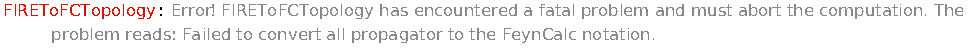
\includegraphics[width=0.6\linewidth]{img/0z6bsy6lc1psd.pdf}
\end{figure}
\FloatBarrier

\begin{dmath*}\breakingcomma
\text{\$Aborted}
\end{dmath*}
\end{document}
